% Author: Till Tantau
% Source: The PGF/TikZ manual
\documentclass{minimal}
\usepackage{tikz}
\usepackage{fullpage}
\usepackage[latin1]{inputenc}
\usetikzlibrary{shapes,arrows}

%\usetikzlibrary{trees,snakes}
\begin{document}
\pagestyle{empty}
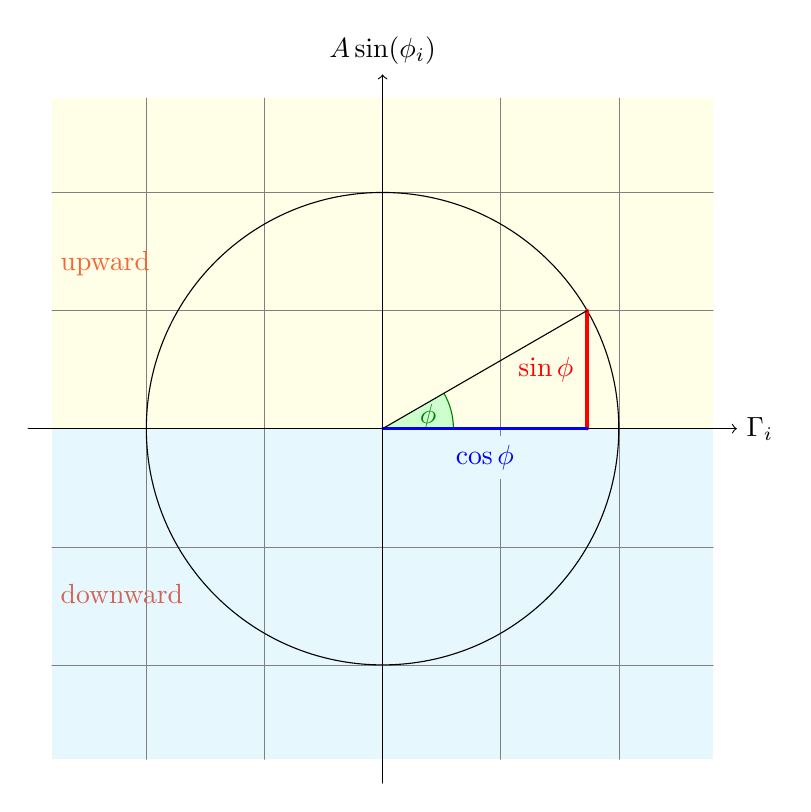
\begin{tikzpicture}[scale=3,cap=round]
  % Local definitions
  \def\costhirty{0.8660256}

  % Colors
  \colorlet{anglecolor}{green!50!black}
  \colorlet{sincolor}{red}
  \colorlet{tancolor}{orange!80!black}
  \colorlet{coscolor}{blue}

  % Styles
  \tikzstyle{axes}=[]
  \tikzstyle{important line}=[very thick]
  \tikzstyle{information text}=[rounded corners,fill=red!10,inner sep=1ex]
 \tikzstyle{rect} = [rectangle, draw=none, ,text width=1em, text centered, ,minimum width=8.4cm,minimum height=4.2cm]

  % The graphic
  \node [draw=none,fill=none](center) {}; 

  \node at (0,0.7) [rect, fill=yellow!10] (back_up){}; 
  \node at (0,-0.7) [rect, fill=cyan!10]  (back_do){}; 
 
  

  \draw[style=help lines,step=0.5cm] (-1.4,-1.4) grid (1.4,1.4);

  \node [draw=none,fill=none, node distance = 4cm,  left of=back_up, text width=.5em, yellow!20!red!80](F_FR) {upward}; 
  \node [draw=none,fill=none, node distance = 4cm,  left of=back_do, text width=.5em, cyan!20!red!80](F_FL) {downward};
  
  \draw (0,0) circle (1cm);

  \begin{scope}[style=axes]
    \draw[->] (-1.5,0) -- (1.5,0) node[right] {$\Gamma_i$};
    \draw[->] (0,-1.5) -- (0,1.5) node[above] {$A\sin(\phi_i)$};

  \end{scope}

  \filldraw[fill=green!20,draw=anglecolor] (0,0) -- (3mm,0pt) arc(0:30:3mm);
  \draw (15:2mm) node[anglecolor] {$\phi$};

  \draw[style=important line,sincolor]
    (30:1cm) -- node[left=1pt,fill=yellow!10] {$\sin\phi$} +(0,-.5);

  \draw[style=important line,coscolor]
    (0,0) -- node[below=2pt,fill=cyan!10] {$\cos \phi$} (\costhirty,0);


  \draw (0,0) -- (0.8660256,0.5);



\end{tikzpicture}

\end{document}